\subsection{Challenge 2: Requirements Refinement}

When systems are decomposed into components, deriving the component requirements from the system requirements is a challenging task. While formal tools help to automatically verify the sufficiency of component requirements to guarantee the system level requirement, deriving and formalizing those component requirements has been a manual activity. Unfortunately, it is has been possible to derive and formalize a set of incorrect and/or infeasible component requirements that the formal tools will verify successfully~\cite{gacek2015towards}.

In an effort to provide guidance to engineers performing and formally verifying the system decomposition, Miller et al~\cite{Miller01:dasc} propose that most system requirements can be recaptured into identical software requirements by slightly modifying the scope of the requirement. Their approach is based on the famous four variable model~\cite{Parnas91:four-variable} that formally captures the high level artifacts of a typical process control system, the requirements ($REQ$), the sensor functions($IN$), controller functions($SOF$), actuator functions ($OUT$) and their environment ($NAT$). The main contribution of the four variable model is mathematically defining the artifacts, their scope (the four variables - \textbf{mon}itored, \textbf{con}trolled, \textbf{in}put and \textbf{out}put used to express the artifacts) and their inter-relationships required to reason about their correctness. Miller et. al extended the four variable model, as shown in Figure~\ref{fig:extn-four-var}. They recreate virtual versions of the variables $mon'$ and $con'$ that differ from the original $mon$ and $con$ in terms of value and timing introduced when sensing and setting the input and output variables. Using these virtual variables, they ``stretch'' the $SOF$ (software) relationship into $IN'$, $REQ'$, and $OUT'$. The $IN'$ and $OUT'$ represents the specification of hardware drivers that were previously part of the $SOF$. With this change, they propose a mere recapture of each function in $REQ$ to $REQ'$ using corresponding variables. They assert that this makes the tracing of the requirements REQ to the software ($REQ'$) direct and straightforward. While this approach superficially seems indisputable and makes the task of decomposition simpler, in our experience, we found that this approach could result in inaccurately specified and verified component requirements.
\vspace{-0.1in}
\begin{figure}[h!]
    \centering
    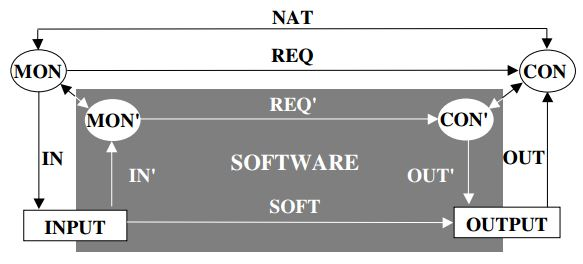
\includegraphics[scale=0.5] {images/FourVarExtn.jpg}
    \caption{Extension of Four Variable Model}
    \label{fig:extn-four-var}
 \end{figure}
\vspace{-0.1in}

The overall system requirements especially for complex control systems such as GPCA are typically captured in such a way to accommodate certain degree of inaccuracies and imperfections, that is they are inherently relational. For example, consider a system level requirement:

\begin{quotation}
\emph{``In basal mode, the system shall infuse the drug at a flow rate within $basal\_flow\_rate$ $\pm t$\% tolerance''}
\end{quotation}

The tolerance (t) in this requirement was included to accommodate inaccuracies of the physical components that is going to be used in the GPCA. When we wanted to identify software requirements of the GPCA, we followed the above guidance and formalized the software requirements in a way that mirrors the system requirement but in terms of inputs and outputs of the software, such as:
\\\\
\footnotesize{\texttt{
(Mode = basal) $\Rightarrow$\\
\textcolor{white}{------}FlowRate $\leq$ (1 + t/100) $\ast$ (BasalFr) and \\
\textcolor{white}{------}FlowRate $\geq$ (1 - t/100) $\ast$ (BasalFr)\\
}}
\normalsize{}\\
While the above formulation appears to be correct as per the guidance, the tolerance part was not intended to be allocated to the software. When we verified requirement it was successfully verified since the software indeed satisfies the requirement, but in an unintended fashion. In reality, the software's output is deterministic and there was no need for the tolerance, hence the consequent in the formalization was supposed to be \texttt{(FlowRate $=$ BasalFr)}. That is, mathematically the requirement of the software is a function as opposed to the system level requirement that is a relation. %In our opinion, failing to understand these differences in mathematical formulation leads to inaccurate understanding of formal verification.

While superficially this doesn't appear to be a problem, an indepth analysis revels that this mere recapture presumes an implicit assumption that the  physical components of the GPCA are perfect. This could lead to a situation in which if the software is compositionally verified in its environment (with physical components) it would fail. The way we formalized the software requirement is not only an over approximation of the capabilities of the software but also masks the other component requirements. While we were able to formally verify if the sub-components satisfies the software requirements, the correctness of the requirements allocated to the software was not formally establishable, since they were originally derived from informal system requirement. Unfortunately, the error in the requirements allocation described was not apparently visible until we started documenting an argument about how software requirements realizes the system level requirements.

\subsubsection {Solution : Satisfaction Argument}
To identify issues with the requirements allocation we propose documenting \emph{satisfaction argument} between each system (or component) requirement and its allocated component (or sub-component) requirements at adjacent levels in the hierarchy, that captures the relationship between them as well the assumptions that are necessary to establish that relationship. This sort of argument, that is inspired from Hammond's work~\cite{Hammond01:WiW}, helped us understand the role of each component in satisfying the system requirement for GPCA. In fact, by documenting the argument we were able to validate the assumptions made for each requirement that consequently helped identify 8 incorrectly formalized component requirements of the GPCA software. While this documentation is straightforward when it is done at the time of requirements allocation, establishing the traceability between the requirements and its assumptions after all requirements are allocated might be laborious. To address that concern, we are currently working towards building an automated traceability capability in the AGREE tool. This capability would automatically identify for every system requirement (parent level) the set of child component requirements that contributed to satisfying it. The task left for the developer is analyze document the traceability and validate it. While we acknowledge that, if one could formally models and specifies requirements of every component of the system, we could use the tools to analyze the composition and identify the requirement errors. However, in practice, whenever informality is involved we recommend documenting a satisfaction argument for every requirement to validate the requirements flow down and assumptions. 